\chapter{NoSQL Graphs Databases}

NoSQL is a movement borned in response to SQL movement. 
Relational Databases have difficult in managing \textbf{Big Data} (bigger data volume, more rapidly changing and more structural variety), for that reasons NoSQL movement is borned. 

There are 4 types of NoSQL movements: 
\begin{itemize}
    \item \textbf{Graph Based}
    \item Key-Value stores
    \item Document-Based
    \item Column Oriented
\end{itemize}

Graph Based movement in turn are divided in two: 
\begin{itemize}
    \item Graph Databases (Neo4j)
    \item RDF Databases
\end{itemize}

\section{Graph Databases}

A graph database is a database that uses the graph structure with nodes, edges and graph properties to represent and store data. \\
\\
A management system (eg Neo4j) offers \textbf{CRUD} operations (Create, Read, Update and Delete) to acces and manipulate data.\\
\\
Graph databases are \textbf{schemaless} $\implies$ you can accumulate data without the need of a predefined rigid schema. You can add new nodes and new edges thanks to the preperty of graphs. \\
\\
Graph databases can be \textbf{queried} through declarative languages, they can provide very good performances because essentially the avoid classic \texttt{joins}. 

\newpage
\subsection*{Relational DB vs Graph DB}

\textbf{Target:} Modeling friends of friends in a relational database. 

\begin{figure}[htbp]
  \centering
  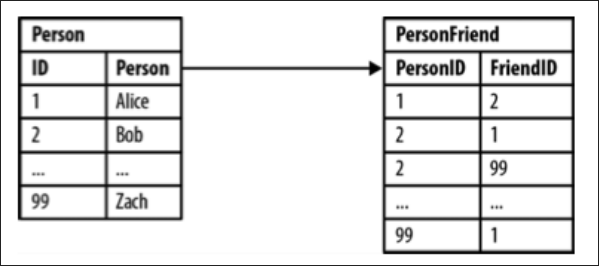
\includegraphics[scale = 0.5]{Attachments/image.png}
  %\caption{${2 didascalia}}
  %\label{fig:${3 etichetta}}
\end{figure}

\begin{figure}[htbp]
  \centering
  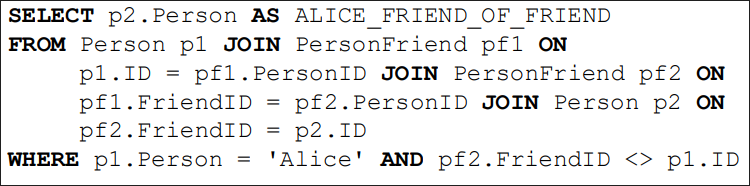
\includegraphics[scale = 0.5]{Attachments/image copy.png}
  %\caption{${2 didascalia}}
  %\label{fig:${3 etichetta}}
\end{figure}

The performances higly deteriorates when we go more in depth into the network of friends. 

\newpage
\textbf{In the graph databases} we can model the relation friend and friend of friend in this way: 

\begin{figure}[htbp]
  \centering
  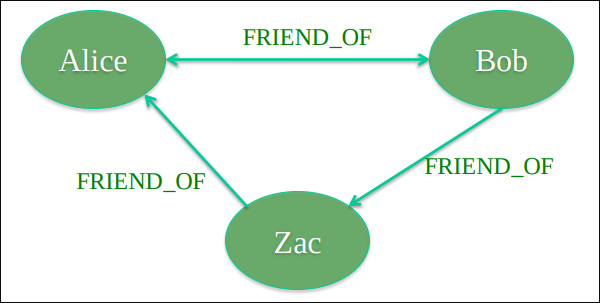
\includegraphics[scale = 0.5]{Attachments/image copy 2.png}
  %\caption{${2 didascalia}}
  %\label{fig:${3 etichetta}}
\end{figure}

Relationship in a graph naturally form paths $\implies$ Querying means actuall \textbf{traversing the graph}. 

\begin{figure}[htbp]
  \centering
  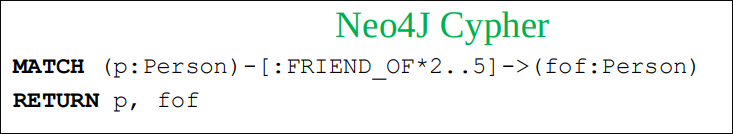
\includegraphics[scale = 0.5]{Attachments/image copy 3.png}
  \caption*{Syntax of Neo4j language for querying}
  %\label{fig:${3 etichetta}}
\end{figure}

\textbf{GraphDB vs Relational DB - Queries}
\begin{itemize}
    \item \textit{Relational DB:} The \texttt{join} operation forms a graph that is dYnamically constructed as one table linked to the other. The limitation is that the graph is not in explicit in the relational structure. 
    \item \textit{Graph DB:} There is no explicit join operation because vertices mantain direct references to their adjacent edges.The edges of the graph serve as explicit, "hard wired" join structure. Traversing (querying) the graph is a \textbf{constant} time operation 
\end{itemize}

